\section{Data Fidelity}
\label{evaluation-sec-fidelity}

The final and most important measure of our network is its ability to provide
scientifically-meaningful data on the volcano's activity. In this section, we
perform an initial analysis of the seismic and acoustic signals from a
seismological perspective, with the goal of validating the accuracy of the
signal quality and timing.

\subsection{Acoustic Wave Propagation}

The infrasonic (low-frequency acoustic) waves generated by the volcano are
primarily the result of explosive events. We start by measuring the velocity
of infrasonic waves recorded by our network, which is more straightforward
than seismic analysis for several reasons. First, infrasonic waves generate a
clear impulse in the microphone signal, making it easy to determine the time
of the wave arrival at each sensor. In addition, acoustic waves propagate
about an order of magnitude more slowly than seismic waves (roughly 340~m/s
versus 1500-4000~m/s). We also expect an infrasonic wave to originate at the
vent of the volcano, simplifying the wave velocity calculation.

\begin{figure}[t]
\begin{center}
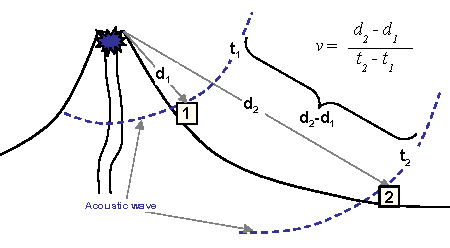
\includegraphics[width=\hsize]{./3-evaluation/figs/acousticsketch.pdf}
\end{center}

\caption{\textbf{Computing acoustic wave velocity.} The velocity of the
acoustic wave is calculated based on the distance of each station from the
vent, $d_i$, and the arrival time of the wave at each station, $t_i$.}

\label{evaluation-fig-acousticsketch}
\end{figure}

We identified four events in our data set with a clear infrasonic component.
For each event, we hand-picked the arrival time of the wave at each node
using the time-rectified signal. Figure~\ref{evaluation-fig-acousticarrival}
plots the wave arrival time versus the distance of each node from the vent.
As shown in Figure~\ref{evaluation-fig-acousticsketch}, the velocity of the
wave can be calculated by performing a linear regression on this dataset.

\begin{figure}[t]
\begin{center}
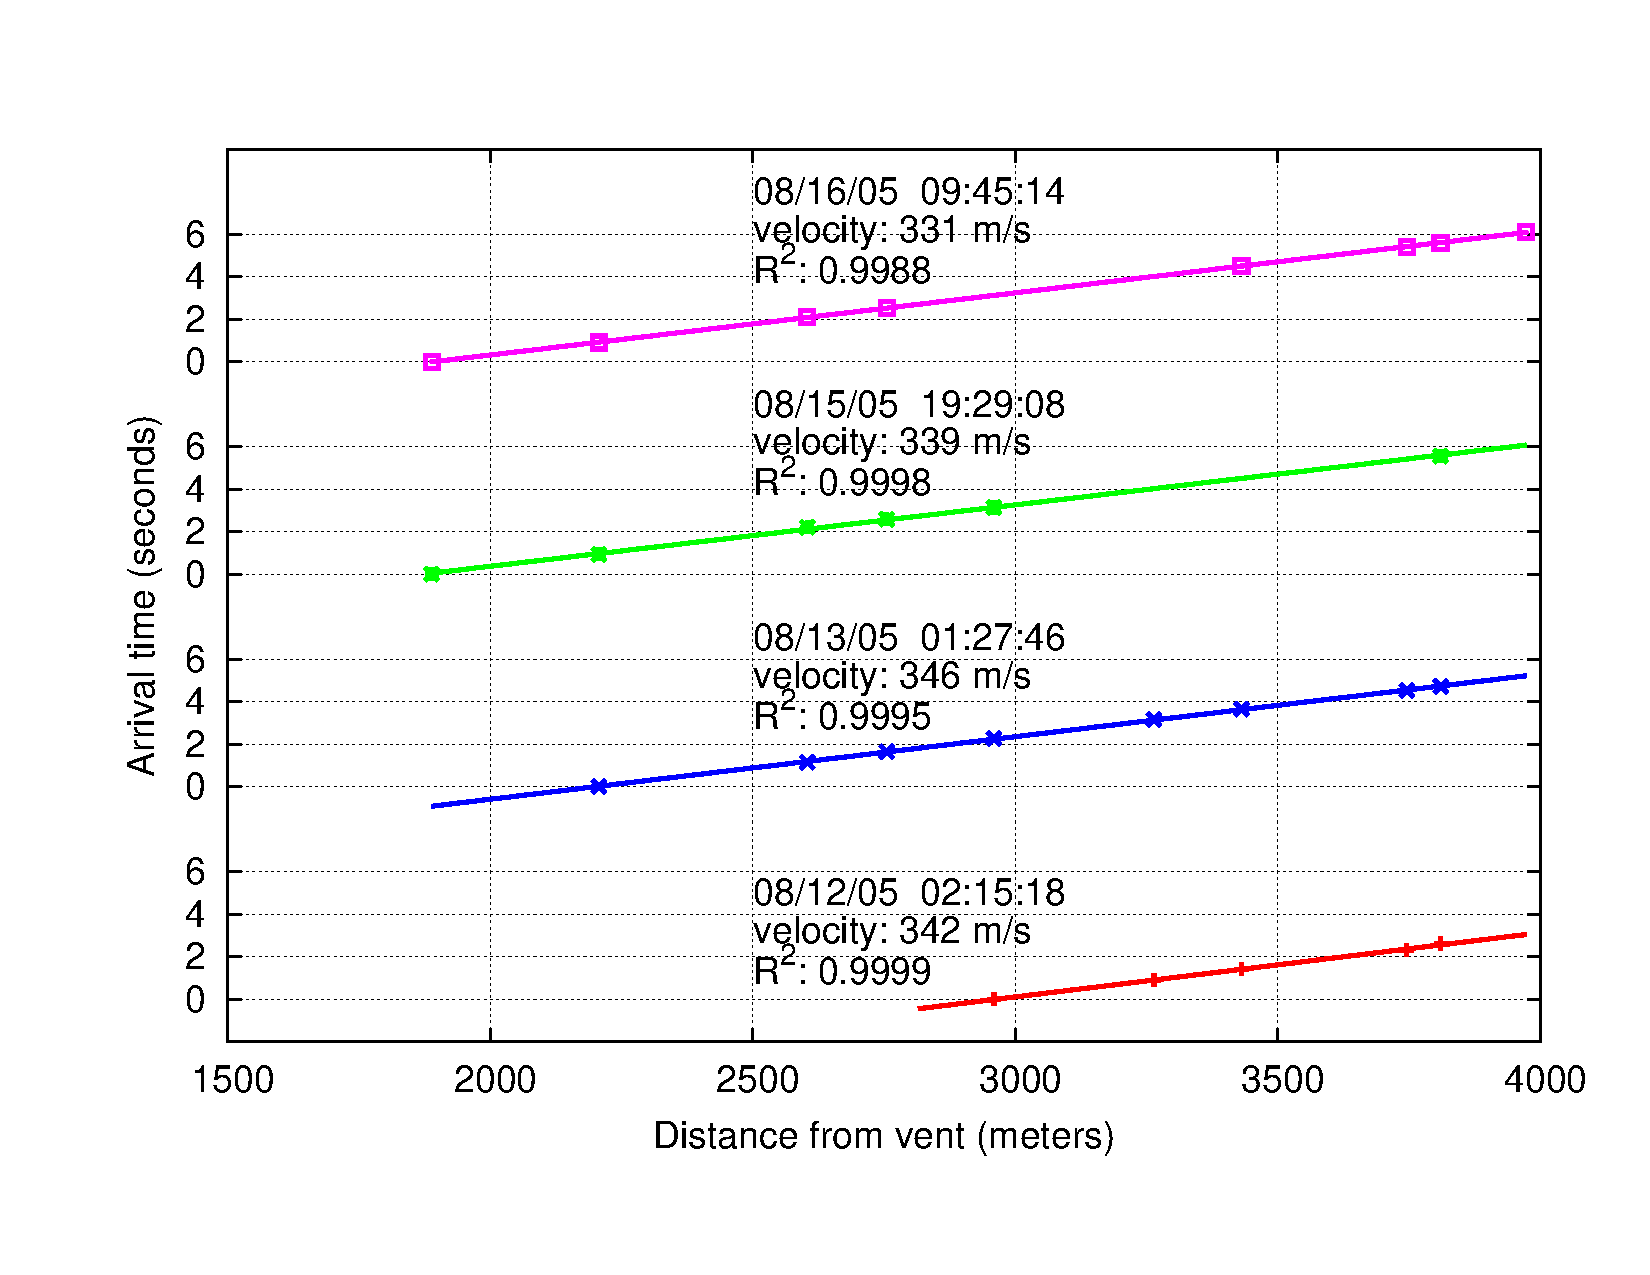
\includegraphics[width=\hsize]{./3-evaluation/figs/acousticarrival.pdf}
\end{center}

\caption{\textbf{Acoustic wave arrival times and velocity.} This figure shows
the acoustic wave arrival time vs. distance from the vent for 4~separate
events. Also shown is the resulting acoustic wave velocity and the $R^2$
coefficient of determination.}

\label{evaluation-fig-acousticarrival}
\end{figure}

The result of this calculation is also shown in
Figure~\ref{evaluation-fig-acousticarrival}. The velocity of sound in air is
temperature-dependent; for temperatures between 10--20 $^{\circ}$C the
velocity range is 337--343~m/s. The calculated wave velocities are mostly in
this range, with a mean of 339.5~m/s. The coefficients of determination $R^2$
are very high, between 0.9988~and~0.9999, showing that the timing and quality
of the acoustic data closely matches our expectation of the infrasonic waves
produced by the volcano.

\subsection{Seismic Wave Propagation}

Analyzing the seismic waves captured by our network is significantly more
challenging. This is primarily because the source locations of seismic waves
are unknown. Seismic events may originate at the vent (in the case of an
explosion) or deep within the edifice, producing very different patterns of
P-~and S-wave arrivals at each node. A full seismological analysis of our
data is beyond the scope of this chapter. However, we present a high-level
measure of the \textit{consistency} of the signals captured by our network:
that is, we evaluate whether the seismic wave arrivals are consistent with
expected volcanic activity.

\begin{figure}[t]
\begin{center}
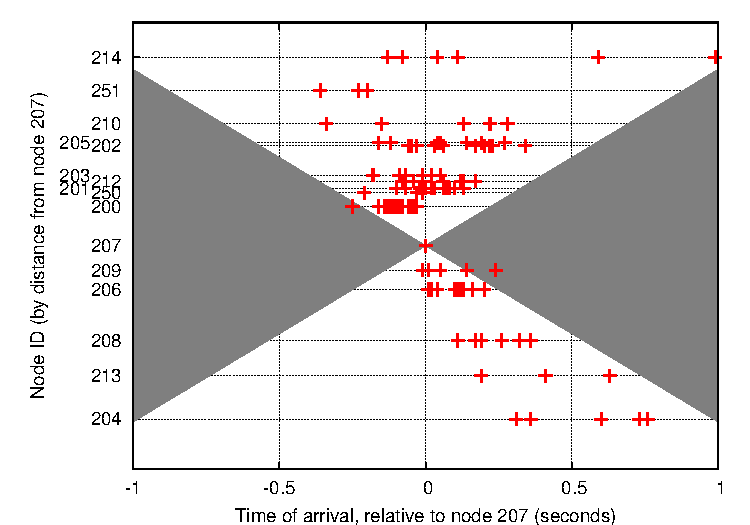
\includegraphics[width=0.8\hsize]{./3-evaluation/figs/arrivaltimes.pdf}
\end{center}

\caption{\textbf{Time of arrival of each node over multiple events.} This
graph shows the spread of arrival times for each node. The arrival time and
distance is relative to Node~207. The arrival time for each node is fairly
consistent over multiple events, with the exception of Node~214. The shaded
area indicates a move-out velocity of less than 1,500 $m/s$.}

\label{evaluation-fig-arrivaltimes}
\end{figure}

The most natural measure of data consistency is whether the time of the
seismic P-wave arrival at each sensor falls within an expected
\textit{envelope} based on the minimum speed at which seismic waves are
believed to propagate at Reventador, which the seismologists estimated at
1500~m/s. We took 15~seismic events with clear P-wave arrivals and used an
automatic algorithm~\cite{pwave-picking} to determine the wave arrival time.
Unlike acoustic waves, determining seismic wave arrival times is notoriously
difficult. The seismograms in Figures~\ref{evaluation-fig-explosionfit} and
Figure~\ref{evaluation-fig-tectonicfit} should give the reader some
appreciation for this.

\begin{figure}[t!]
\begin{center}
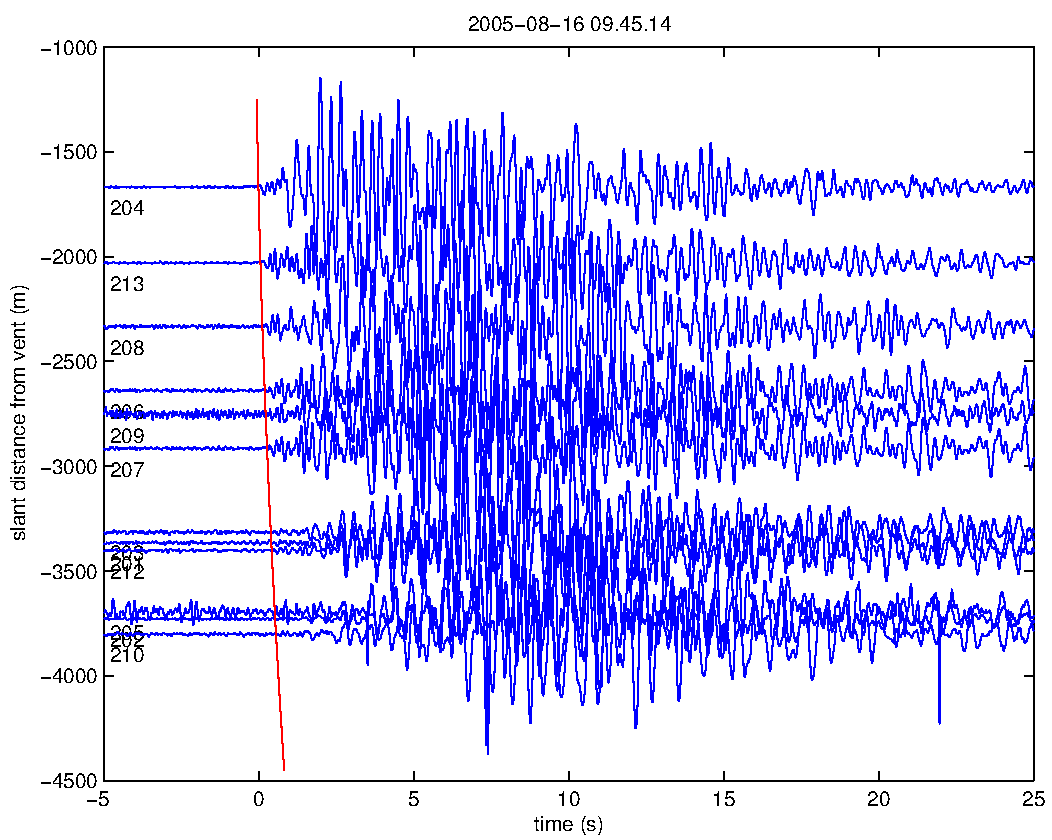
\includegraphics[width=0.8\hsize]{./3-evaluation/figs/explosionfit.pdf}
\end{center}

\caption{\textbf{Explosion earthquake event.} P-wave arrivals have been
identified manually and a second-order polynomial (solid line) is fit to the
arrivals. The arrival time move-outs are consistent with a shallow near-vent
source.}

\label{evaluation-fig-explosionfit}
\end{figure}

Figure~\ref{evaluation-fig-arrivaltimes} shows a scatterplot of the arrival
times with respect to Node~207, which was chosen as an arbitrary reference
point since data for this node appeared in all 15~events. The $y$-axis
represents the distance of each node from Node~207. Depending on the seismic
source location, we expect waves to arrive both before and after Node~207.
However, the slowest wave speed (1500~m/s) dictates the maximum difference in
the wave arrival between each station. Note that there is no lower bound on
arrival times, since a wave emanating from a deep source could arrive at all
stations nearly simultaneously. The shaded area in
Figure~\ref{evaluation-fig-arrivaltimes} covers the ``exclusion envelope'' of
arrival times at each station. As the figure shows, only 2~out of~124
arrivals fall outside of this envelope.

Finally, we take a closer look at two seismic events recorded by our array.
Figures~\ref{evaluation-fig-explosionfit} and
\ref{evaluation-fig-tectonicfit} show seismograms from each of the sensor
nodes after time rectification. The $y$-axis corresponds to the distance of
each node from the vent. For each event, the P-wave arrivals have been
determined by hand and a second-order polynomial has been fit to the arrival
times at each node for clarity.

These two events show a very different pattern of wave arrival times.
Figure~\ref{evaluation-fig-explosionfit} shows the seismic wave arriving
first at stations near the vent (nodes~204 and 213). This is consistent with
a shallow near-vent source corresponding to an explosion. This is confirmed
by the corresponding acoustic data (shown in
Figure~\ref{evaluation-fig-acousticarrival}) attributed to explosive
expansion of gas.

In contrast, Figure~\ref{evaluation-fig-tectonicfit} shows an event with the
earliest arrivals in the middle of the sensor array and the endpoints
relatively delayed; many such events were recorded by our network. This
distribution implies a deeper source. At the same time, seismic velocity in
the uppermost cone, which is comprised of unconsolidated volcanic deposits,
is presumed to be slower. Such volcano-tectonic events are likely generated
by the fracturing of solid media typically induced by pressurization within
the edifice. This preliminary study demonstrates the value of our wireless
sensor network for collecting accurate signals that can be subjected to
seismological analysis.

\begin{figure}[t!]
\begin{center}
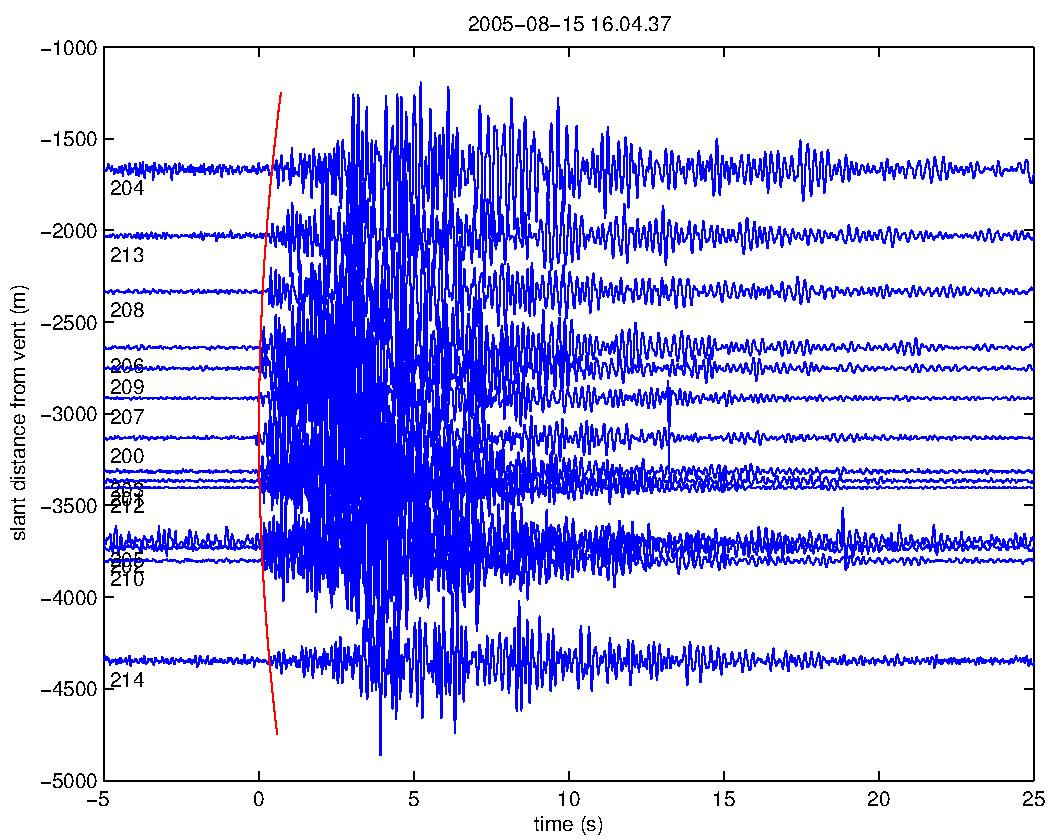
\includegraphics[width=0.8\hsize]{./3-evaluation/figs/tectonicfit.pdf}
\end{center}

\caption{\textbf{Tectonic earthquake event at 08/15/2005 16:04:37 GMT.} In
this event, seismic waves are first recorded near the middle of the sensor
array. This is due either to a source closer to the center of the array,
variations in velocity structure, or most likely both.}

\label{evaluation-fig-tectonicfit}
\end{figure}
